%Version 3 October 2023
% See section 11 of the User Manual for version history
%
%%%%%%%%%%%%%%%%%%%%%%%%%%%%%%%%%%%%%%%%%%%%%%%%%%%%%%%%%%%%%%%%%%%%%%
%%                                                                 %%
%% Please do not use \input{...} to include other tex files.       %%
%% Submit your LaTeX manuscript as one .tex document.              %%
%%                                                                 %%
%% All additional figures and files should be attached             %%
%% separately and not embedded in the \TeX\ document itself.       %%
%%                                                                 %%
%%%%%%%%%%%%%%%%%%%%%%%%%%%%%%%%%%%%%%%%%%%%%%%%%%%%%%%%%%%%%%%%%%%%%

%%\documentclass[referee,sn-basic]{sn-jnl}% referee option is meant for double line spacing

%%=======================================================%%
%% to print line numbers in the margin use lineno option %%
%%=======================================================%%

%%\documentclass[lineno,sn-basic]{sn-jnl}% Basic Springer Nature Reference Style/Chemistry Reference Style

%%======================================================%%
%% to compile with pdflatex/xelatex use pdflatex option %%
%%======================================================%%

%%\documentclass[pdflatex,sn-basic]{sn-jnl}% Basic Springer Nature Reference Style/Chemistry Reference Style


%%Note: the following reference styles support Namedate and Numbered referencing. By default the style follows the most common style. To switch between the options you can add or remove �Numbered� in the optional parenthesis. 
%%The option is available for: sn-basic.bst, sn-vancouver.bst, sn-chicago.bst%  
 
%%\documentclass[sn-nature]{sn-jnl}% Style for submissions to Nature Portfolio journals
%%\documentclass[sn-basic]{sn-jnl}% Basic Springer Nature Reference Style/Chemistry Reference Style
\documentclass[sn-mathphys-num]{sn-jnl}% Math and Physical Sciences Numbered Reference Style 
%%\documentclass[sn-mathphys-ay]{sn-jnl}% Math and Physical Sciences Author Year Reference Style
%%\documentclass[sn-aps]{sn-jnl}% American Physical Society (APS) Reference Style
%%\documentclass[sn-vancouver,Numbered]{sn-jnl}% Vancouver Reference Style
%%\documentclass[sn-apa]{sn-jnl}% APA Reference Style 
%%\documentclass[sn-chicago]{sn-jnl}% Chicago-based Humanities Reference Style

%%%% Standard Packages
%%<additional latex packages if required can be included here>

\usepackage{graphicx}%
\usepackage{multirow}%
\usepackage{amsmath,amssymb,amsfonts}%
\usepackage{amsthm}%
\usepackage{mathrsfs}%
\usepackage[title]{appendix}%
\usepackage{xcolor}%
\usepackage{textcomp}%
\usepackage{manyfoot}%
\usepackage{booktabs}%
\usepackage{algorithm}%
\usepackage{algorithmicx}%
\usepackage{algpseudocode}%
\usepackage{listings}%
%%%%

%%%%%=============================================================================%%%%
%%%%  Remarks: This template is provided to aid authors with the preparation
%%%%  of original research articles intended for submission to journals published 
%%%%  by Springer Nature. The guidance has been prepared in partnership with 
%%%%  production teams to conform to Springer Nature technical requirements. 
%%%%  Editorial and presentation requirements differ among journal portfolios and 
%%%%  research disciplines. You may find sections in this template are irrelevant 
%%%%  to your work and are empowered to omit any such section if allowed by the 
%%%%  journal you intend to submit to. The submission guidelines and policies 
%%%%  of the journal take precedence. A detailed User Manual is available in the 
%%%%  template package for technical guidance.
%%%%%=============================================================================%%%%

%% as per the requirement new theorem styles can be included as shown below
\theoremstyle{thmstyleone}%
\newtheorem{theorem}{Theorem}%  meant for continuous numbers
%%\newtheorem{theorem}{Theorem}[section]% meant for sectionwise numbers
%% optional argument [theorem] produces theorem numbering sequence instead of independent numbers for Proposition
\newtheorem{proposition}[theorem]{Proposition}% 
%%\newtheorem{proposition}{Proposition}% to get separate numbers for theorem and proposition etc.

\theoremstyle{thmstyletwo}%
\newtheorem{example}{Example}%
\newtheorem{remark}{Remark}%

\theoremstyle{thmstylethree}%
\newtheorem{definition}{Definition}%

\raggedbottom
%%\unnumbered% uncomment this for unnumbered level heads

\begin{document}

\title[Supplementary Information: Towards Transparency and Knowledge Exchange in AI-assisted Data Analysis Code Generation]{Supplementary Information: Towards Transparency and Knowledge Exchange in AI-assisted Data Analysis Code Generation}

%%=============================================================%%
%% GivenName	-> \fnm{Joergen W.}
%% Particle	-> \spfx{van der} -> surname prefix
%% FamilyName	-> \sur{Ploeg}
%% Suffix	-> \sfx{IV}
%% \author*[1,2]{\fnm{Joergen W.} \spfx{van der} \sur{Ploeg} 
%%  \sfx{IV}}\email{iauthor@gmail.com}
%%=============================================================%%

\author[1,2]{Robert Haase}
\email{robert.haase@uni-leipzig.de}

\affil[1]{Data Science Center, Leipzig University, Humboldtstra{\ss}e 25, 04105 Leipzig, Germany}
\affil[2]{Center for Scalable Data Analytics and Artificial Intelligence (ScaDS.AI) Dresden / Leipzig}

%%==================================%%
%% Sample for unstructured abstract %%
%%==================================%%

%%\maketitle

\begin{appendices}


%%%%%%%%%%%%%%%%%%%%%%%%%%%%%
% Supplementary Information %
%%%%%%%%%%%%%%%%%%%%%%%%%%%%%
%\captionsetup*{format=largeformat}


\onecolumn
\newpage

\setcounter{figure}{0} 
\renewcommand{\figurename}{}
\renewcommand{\thefigure}{Supplementary Figure \arabic{figure}}


\begin{figure*}[h]
\centering
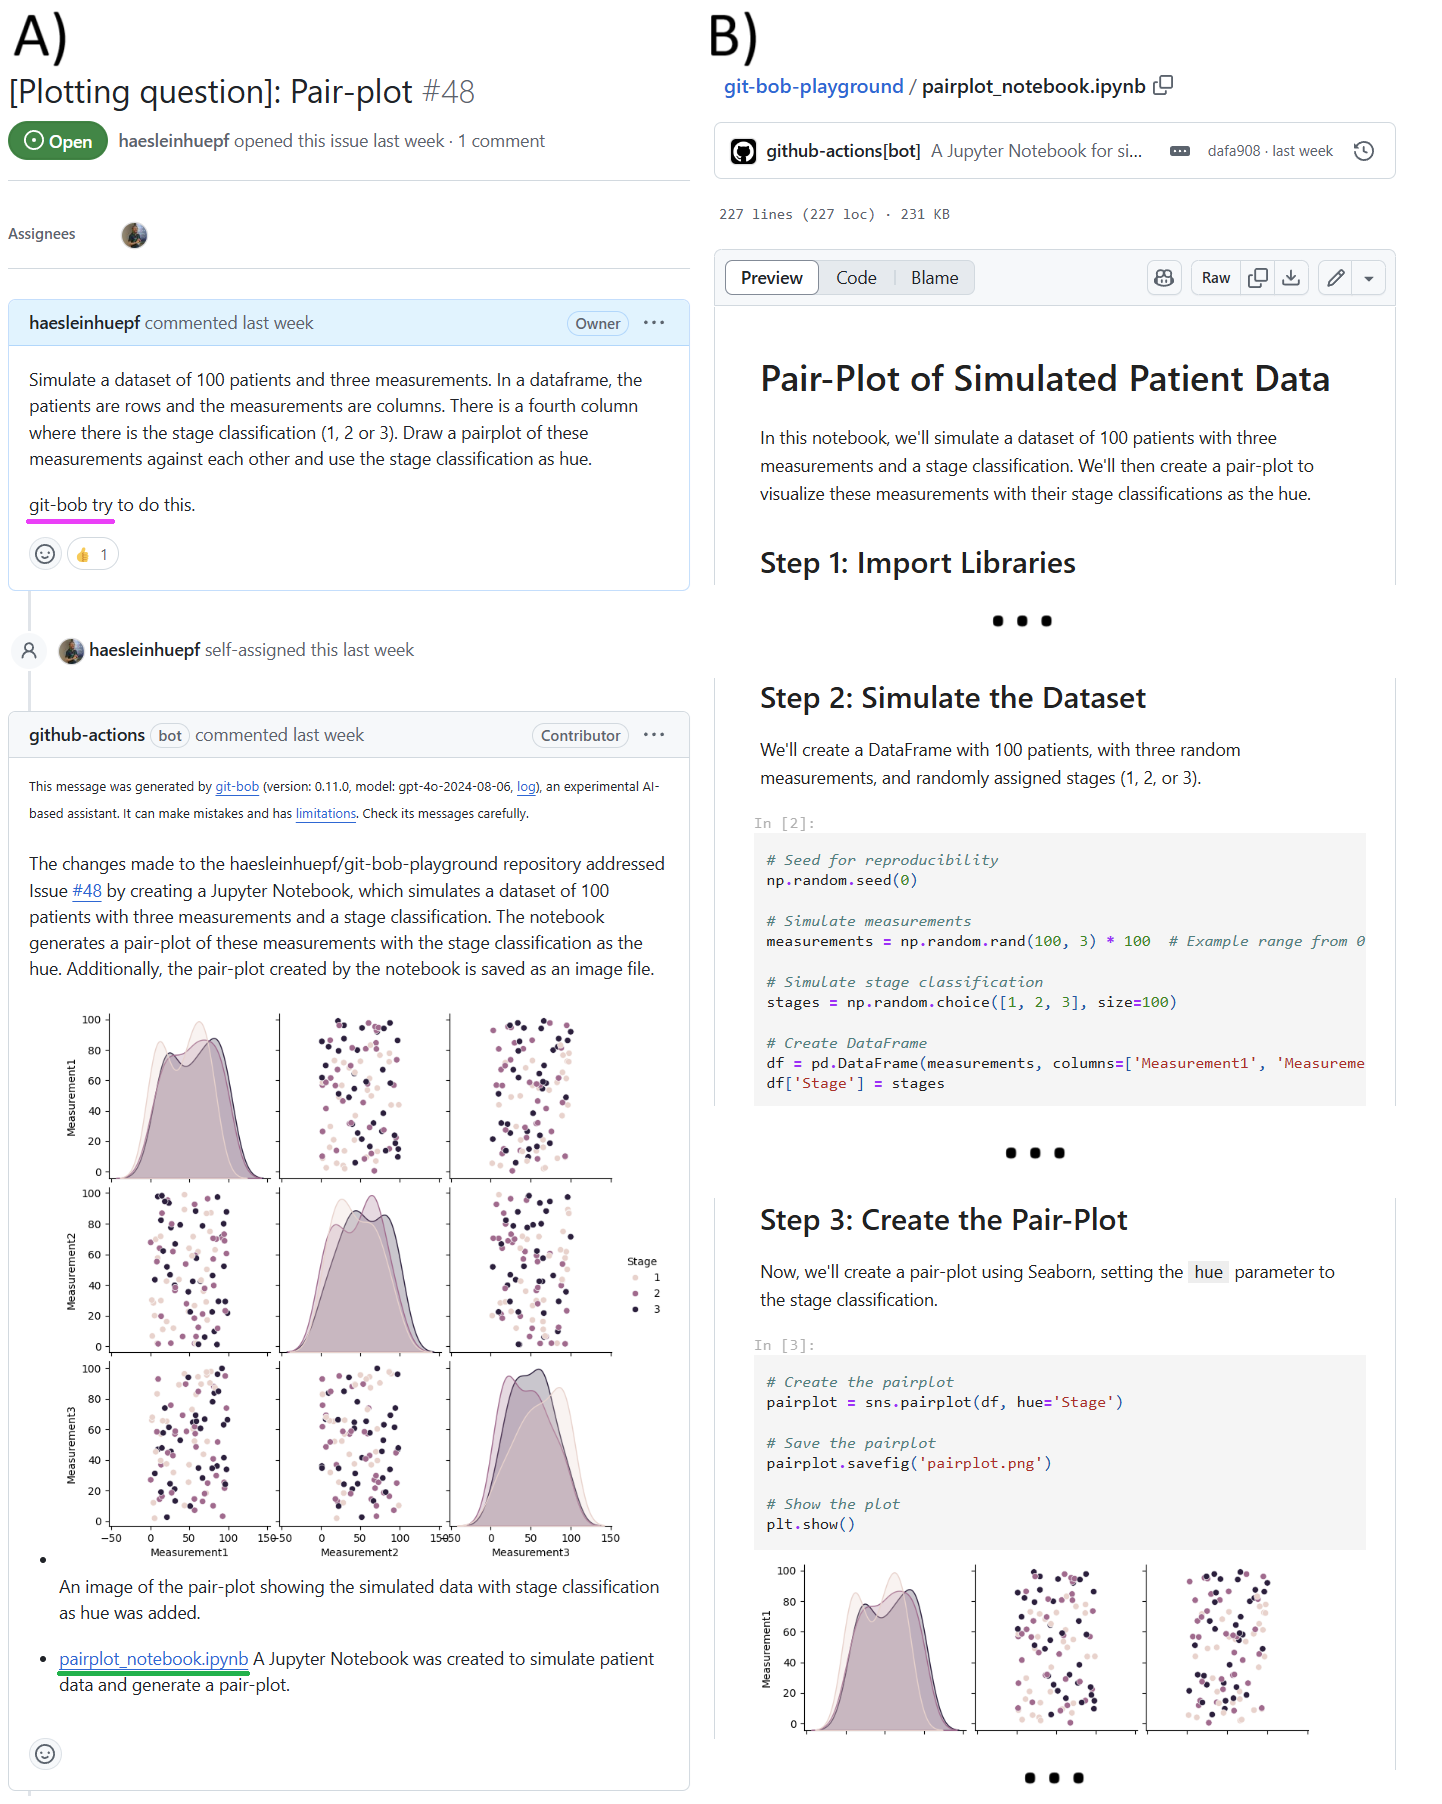
\includegraphics[width=0.9\textwidth]{example_pair_plot.png}
\caption{\textbf{Use-case example for generating data analysis code:} The user explains a scenario (A) and triggers git-bob (underlined in magenta). The AI-assistant generates and executes code and visualizes the resulting plot. The user can click on the link to the generated notebook (underlined in green) to go to the notebook (B) and read the code and see intermediate results. The shown notebook is an excerpt as indicated by ``...''. The entire discussion and corresponding code can be read online: \url{https://github.com/haesleinhuepf/git-bob-playground/issues/48}
\newline
\newline
}
\label{fig:examplepairplot}
\end{figure*}


\begin{figure*}[h]
\centering
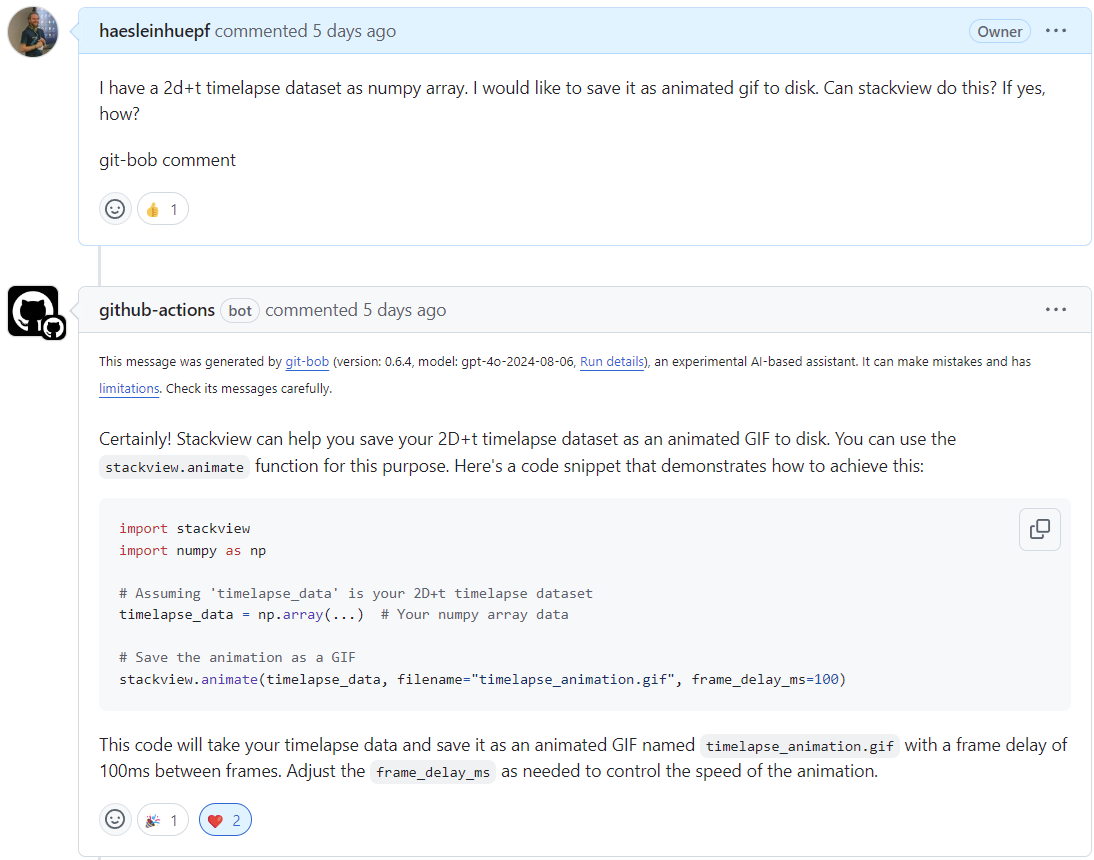
\includegraphics[width=0.8\textwidth]{example_supporting_users.png}
\caption{\textbf{Use-case example for supporting users:} The assistant can be configured to act as expert on a specific Python library and answer user questions. Words triggering git-bob are underlined in magenta. The entire discussion and corresponding code can be read online: \url{https://github.com/haesleinhuepf/stackview/issues/79}
\newline
\newline
}
\label{fig:examplesupportingusers}
\end{figure*}


\begin{figure*}[h]
\centering
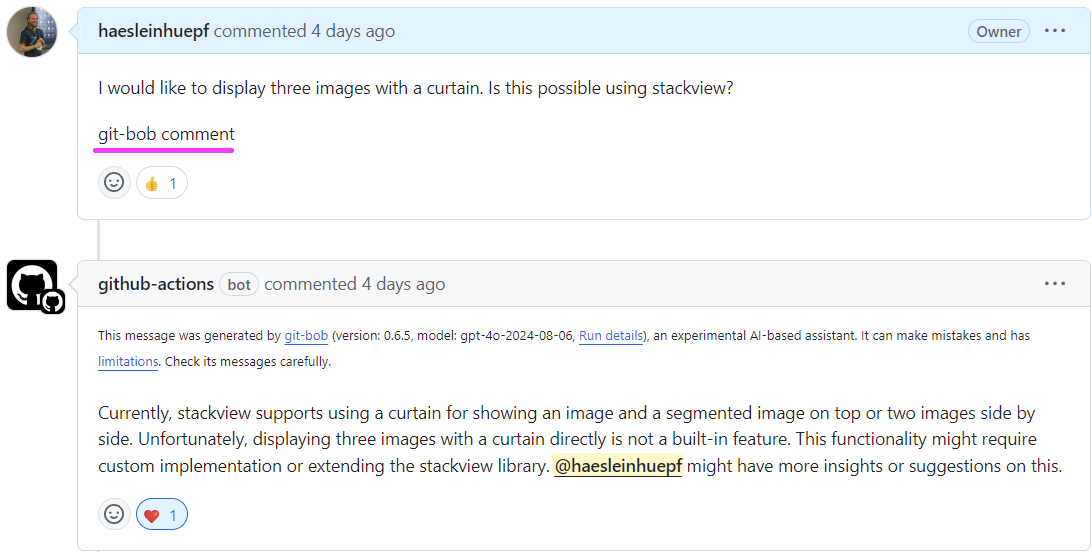
\includegraphics[width=0.8\textwidth]{example_supporting_users2.png}
\caption{\textbf{Use-case example for asking an expert:} The answer to the question shown here is "No", but this is nowhere written in the documentation or the configuration of the assistant. In this case the assistant is not sure, and it can be configured to forward a question to a maintainer of the library where the question arrived. Words triggering git-bob are underlined in magenta. The entire discussion and corresponding code can be read online: \url{https://github.com/haesleinhuepf/stackview/issues/80}
\newline
\newline
}
\label{fig:examplesupportingusers2}
\end{figure*}



\begin{figure*}[h]
\centering
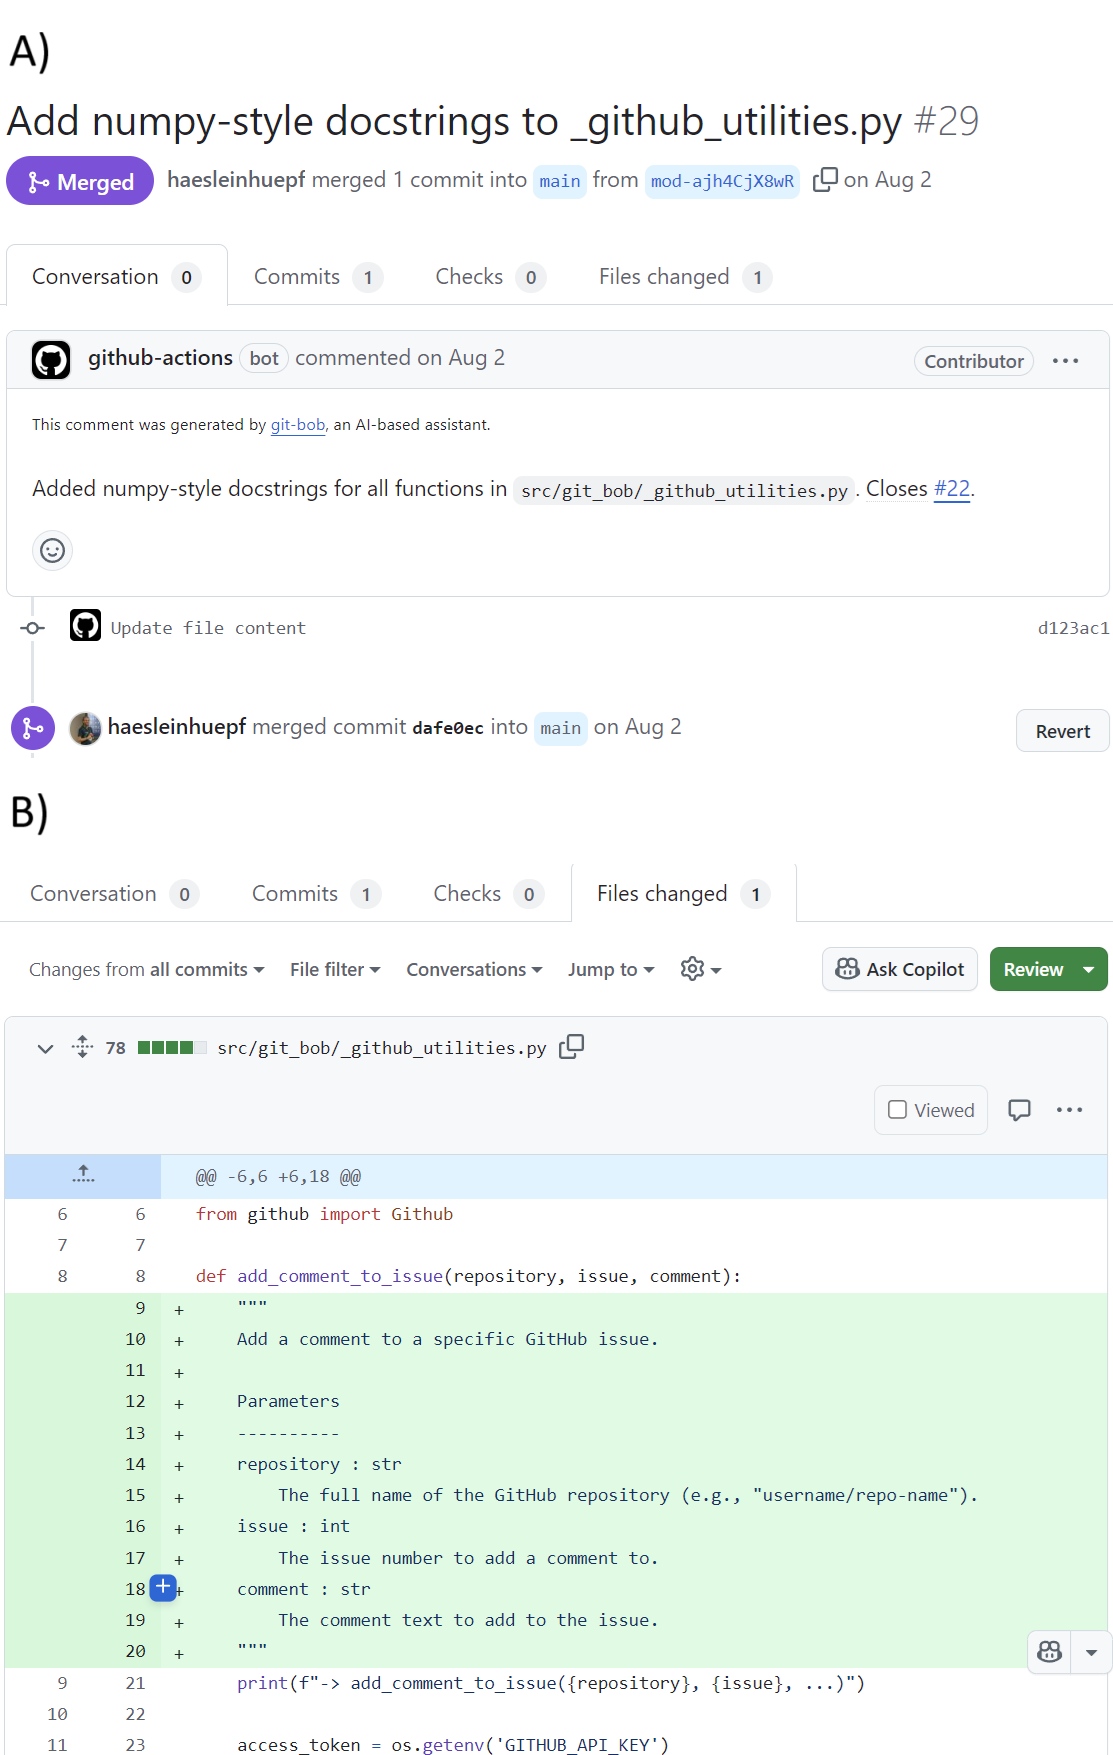
\includegraphics[width=0.82\textwidth]{example_add_documentation.png}
\caption{\textbf{Use-case example for adding and revising documentation in code:} git-bob was used to partially write the code documentation of its own code. When asked to add documentation in a specific format, it sent a pull-request (A) and the human could inspect the code modifications (B, excerpt) before mergin the code into the project's code base. The entire discussion and corresponding code can be read online: \url{https://github.com/haesleinhuepf/git-bob/pull/29}
\newline
\newline
}
\label{fig:example_add_documentation}
\end{figure*}


\begin{figure*}[h]
\centering
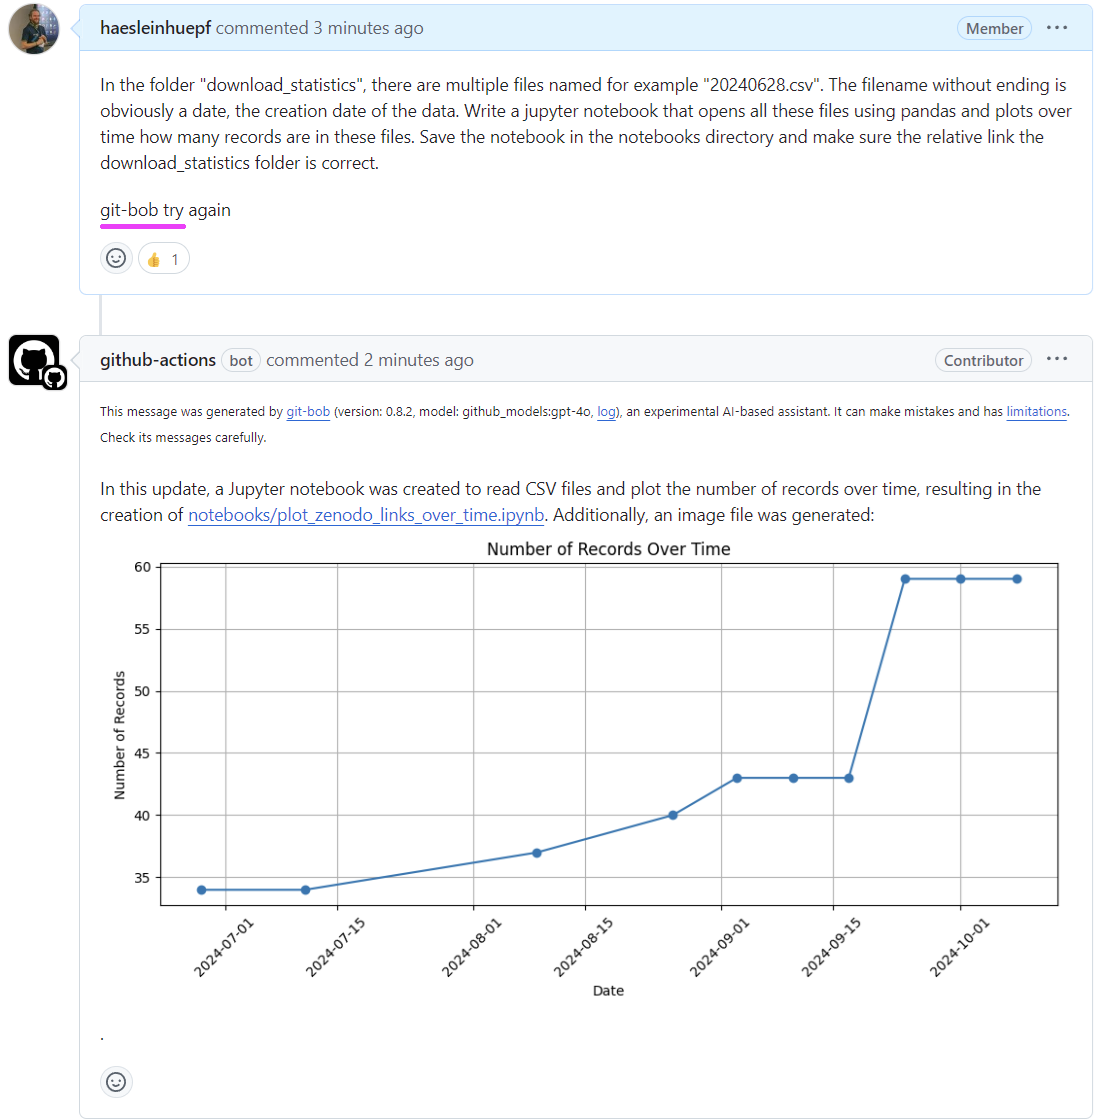
\includegraphics[width=\textwidth]{example_plotting.png}
\caption{\textbf{Use-case example for plotting data:} after explaining the assistant the folder structure of the project, it generates code for parsing a folder of CSV files and plotting results. Words triggering git-bob are underlined in magenta. The entire discussion and corresponding code can be read online: \url{https://github.com/NFDI4BIOIMAGE/training/issues/250}
\newline
\newline
}
\label{fig:exampleplotting}
\end{figure*}






\begin{figure*}[h]
\centering
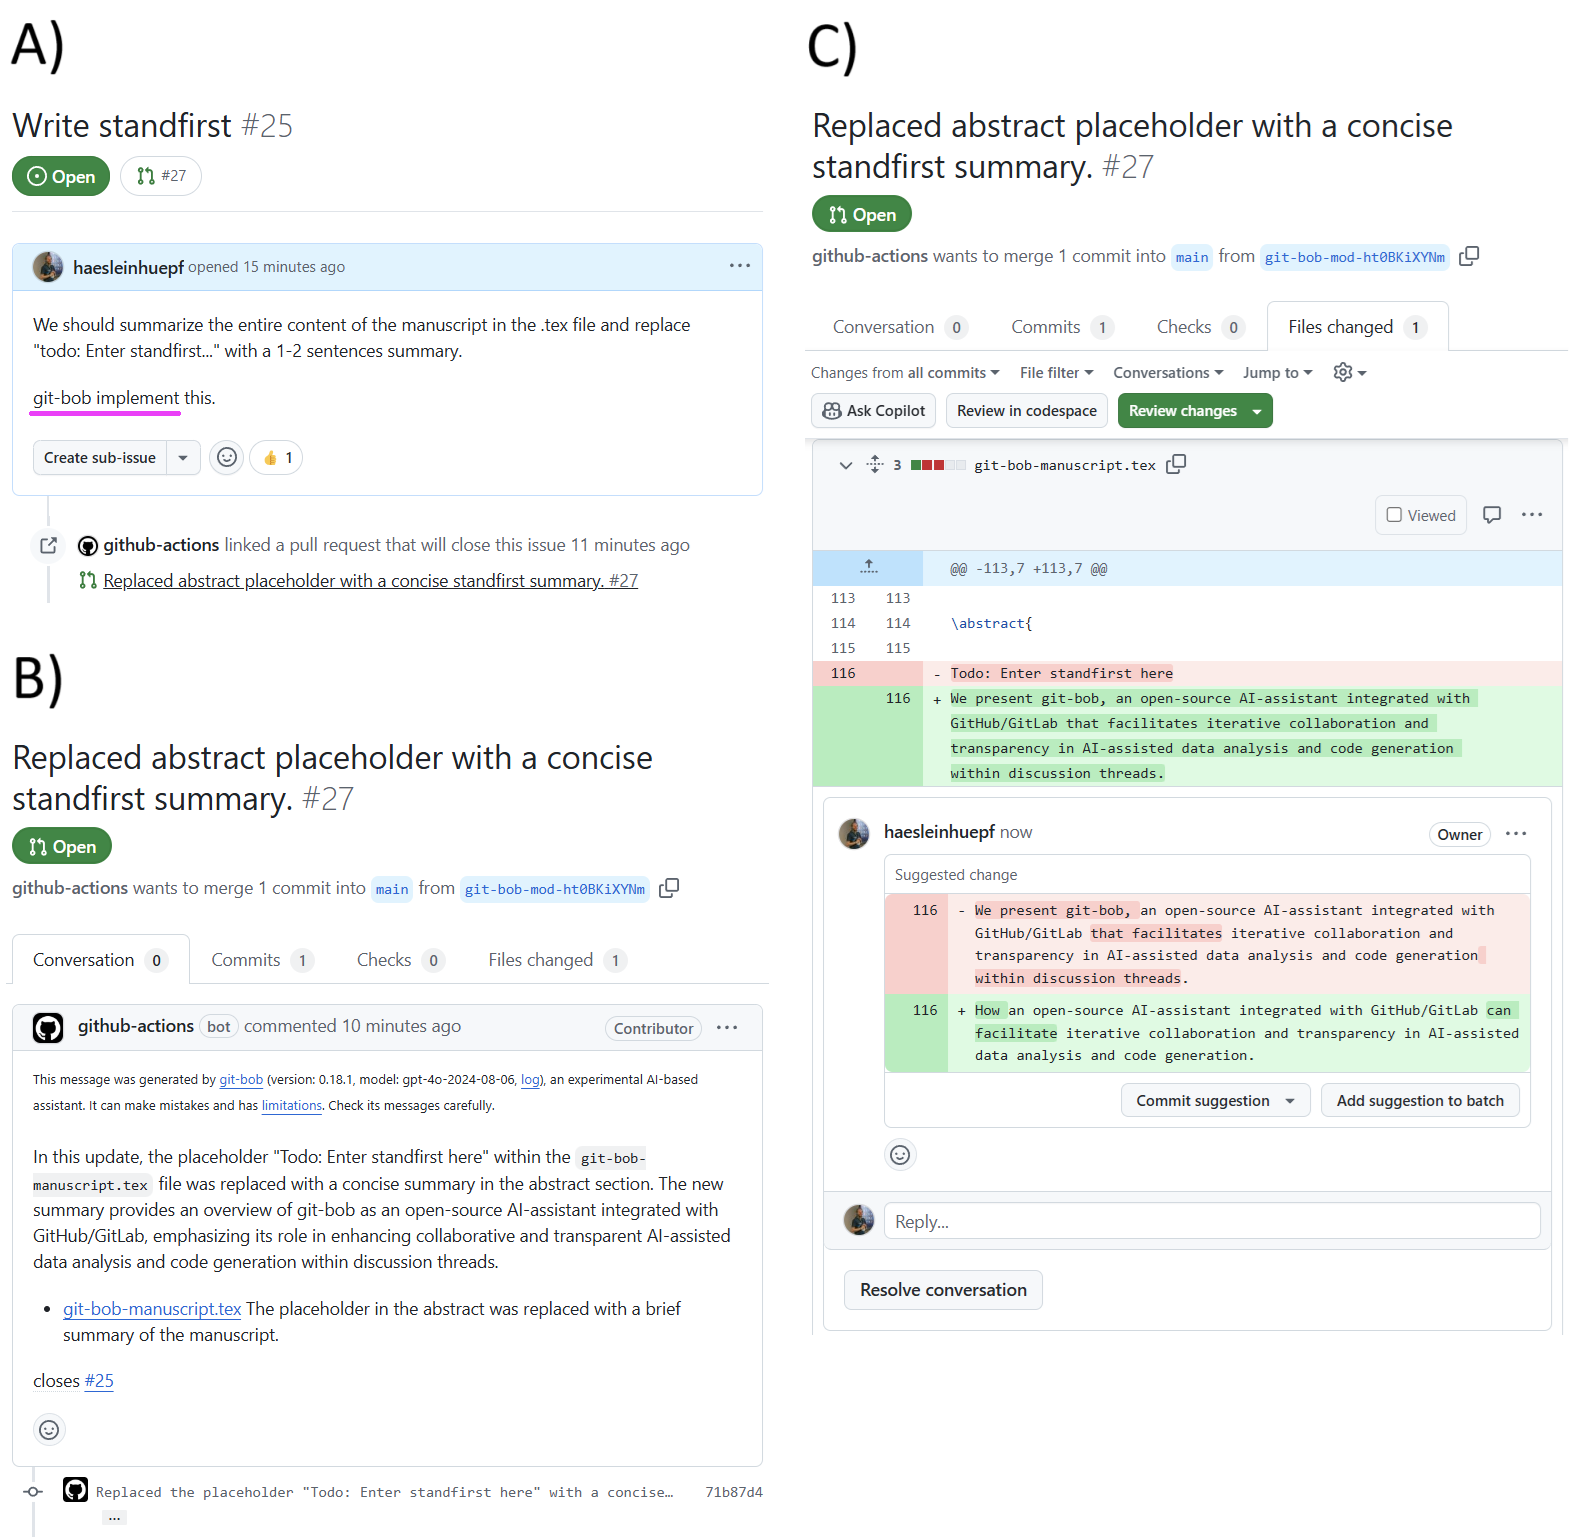
\includegraphics[width=\textwidth]{example_standfirst_generation.png}
\caption{\textbf{Use-case example for working on scientific manuscripts:} after a draft of the manuscript was written, git-bob was asked to formulate an summary (A). The summary was then submitted as pull-request with a short description (B). The human has to review and optionally modify the proposed text in GitHub's online interface (C). Words triggering git-bob are underlined in magenta. The entire discussion can be read online: \url{https://github.com/haesleinhuepf/git-bob-manuscript/issues/25} and \url{https://github.com/haesleinhuepf/git-bob-manuscript/pull/27}.
\newline
\newline
}
\label{fig:xample_abstract_generation}
\end{figure*}

\end{appendices}

%%===========================================================================================%%
%% If you are submitting to one of the Nature Portfolio journals, using the eJP submission   %%
%% system, please include the references within the manuscript file itself. You may do this  %%
%% by copying the reference list from your .bbl file, paste it into the main manuscript .tex %%
%% file, and delete the associated \verb+\bibliography+ commands.                            %%
%%===========================================================================================%%

%%\bibliography{mybibfile}% common bib file
%% if required, the content of .bbl file can be included here once bbl is generated
%%\input sn-article.bbl

%% BioMed_Central_Bib_Style_v1.01



\end{document}

